%\setcounter{chapter}{2}

\chapter{LHC and the CMS experiment}
\label{ch:cms}

\section{The history of the Large Hadron Collider}\label{sec:cms_intro}

CERN accelerator complex is a sequence of machines that produces and accelerates bunches of protons to nearly the speed of light. The process starts with the bottle of hydrogen gas, which acts as a source of protons. The hydrogen atoms are fed into the source chamber of the Linear Accelerator (Linac). There, heat up to high temperatures, electrons are stripped off of the hydrogen atoms. Using the electric field the protons are directed to the first acceleration stage - Linac, which accelerates the protons to the energy of 50 MeV. After Linac, the beam of protons is injected into the Proton Synchrotron Booster (PSB), where the protons are accelerated to 1.4 GeV. The third stage is the Proton Synchrotron (PS), there, the energy of the proton beam is increased to 25 GeV. After that, the protons are sent to the Super Proton Synchrotron (SPS), where they are accelerated to 450 GeV. This is the final pre-LHC stage. 

Large Hadron Collider (LHC) (see Fig. \ref{lhcmap}) is the most powerful particle accelerator that has ever been built. It is located at the border of France and Switzerland at a depth from 50 to 175 m underground. LHC is 26.7 km in circumference and is reutilising the tunnel used previously by the Large Electron Positron collider. 




From the SPS, the proton beam consisting of the proton bunches of $10^11$ protons, with each bunch separated by O(10) m from each other, is injected to two LHC beam pipes. 


Beams in the LHC circulate in the opposite directions and it takes SPS 4 minutes and 20 seconds to fill each LHC ring with bunches. During standard data taking, beams circulate for O(10) hours inside the LHC beam pipes. At four points two beams are brought into collisions -  inside four detectors - ALICE, ATLAS, CMS ,and LHCb. This thesis analyses the data that is produced in proton-proton collisions by LHC at 13 TeV centre-of-mass collision energy.





The story of LHC begins in 1977, when the CERN director general Sir John Adams suggested that LEP tunnel can be reused to accommodate the future hadron collider of more than 3 TeV energies \ref{Sadenius}. At the 1984 ECFA-CERN workshop on a "Large Hadron Collider in the LEP Tunnel" \ref{LHC1984}, the plans for LHC were stated, where the plans for LHC were stated, with the physics goals including the confirmation of the BEH mechanism, search for the Higgs Boson, and exploration of the origin of masses of W and Z bosons. The parameters of the proposed LHC were very ambitious: the centre-of-mass collision energy of 10 to 20 TeV, and a target instantaneous luminosity of 10$^{33-34}\frac{1}{cm^{2}s}$. 



The quantity that measures the ability of a particle accelerator to produce the required number of interactions is called the luminosity and is the proportionality factor between the number of events per second dR/dt and the cross section \cite{Herr:941318}



Luminosity is the coefficient which relates the cross section $\sigma$ of the process to the number of events $N_{events}$ that will be produced in  LHC collisions: $N_{events} = L \sigma$. Luminosity is the parameter controlled by the machine and can be written as:

$L=\frac{N^2 n_b f_{rev}}{4\pi \sigma_x \sigma_y}$

\noindent where $N_b$ is the number of particle in the colliding bunch, $n_b$ is the number of colliding bunches in the beam, $f_{rev}$ is the revolution frequency, 

? ?x,y ?? 11?m is the standard deviation of the beam density profile in the trans-
verse plane (here assumed to be equal for both beams and to follow a Gaussian 
distribution), at the IP and at 13 TeV.

The luminosity is not constant and decays with time due to the degradation of the initial circulating beams. Theoretical decay time to reach $1/e$ level is approximately 29 h. In practice, adding contributions from the intrabeam scattering, scattering on the residual gas, etc, the final luminosity lifetime is measured to be 15 h. 

Another useful variation of the luminosity parameter is a total integrated luminosity. Integrating over the instantaneous luminosity during the run period, one obtains: 

 $L_{int} = L_0 \tau_L \left[  1- e^{\frac{-\tau_{run}}{\tau_L}}  \right]$, 

\noindent where $L_0$ is the initial luminosity, $\tau_run$ is the total duration of the run, and $\tau_L$ is the luminosity lifetime. The optimum run time is 12 hours. 

talk about dumping, clean , etc.

If we denote the area of 10$^{-28}$ $m^2$ as barn (b), then in terms of these new units the LHC can theoretically produce $80-120/fb$ of data a year. 



\begin{figure}[H]
  \centering
  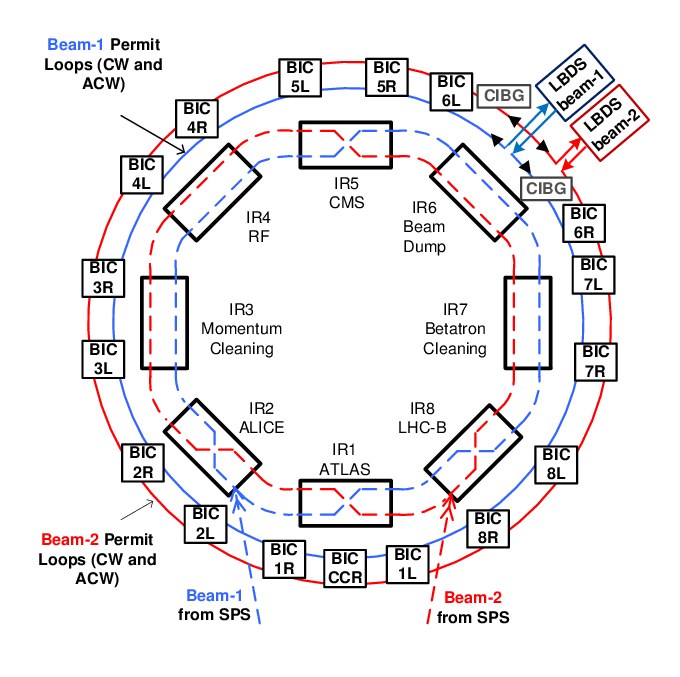
\includegraphics[width=0.75\textwidth]{LHC-beam-permit-loops}\\
  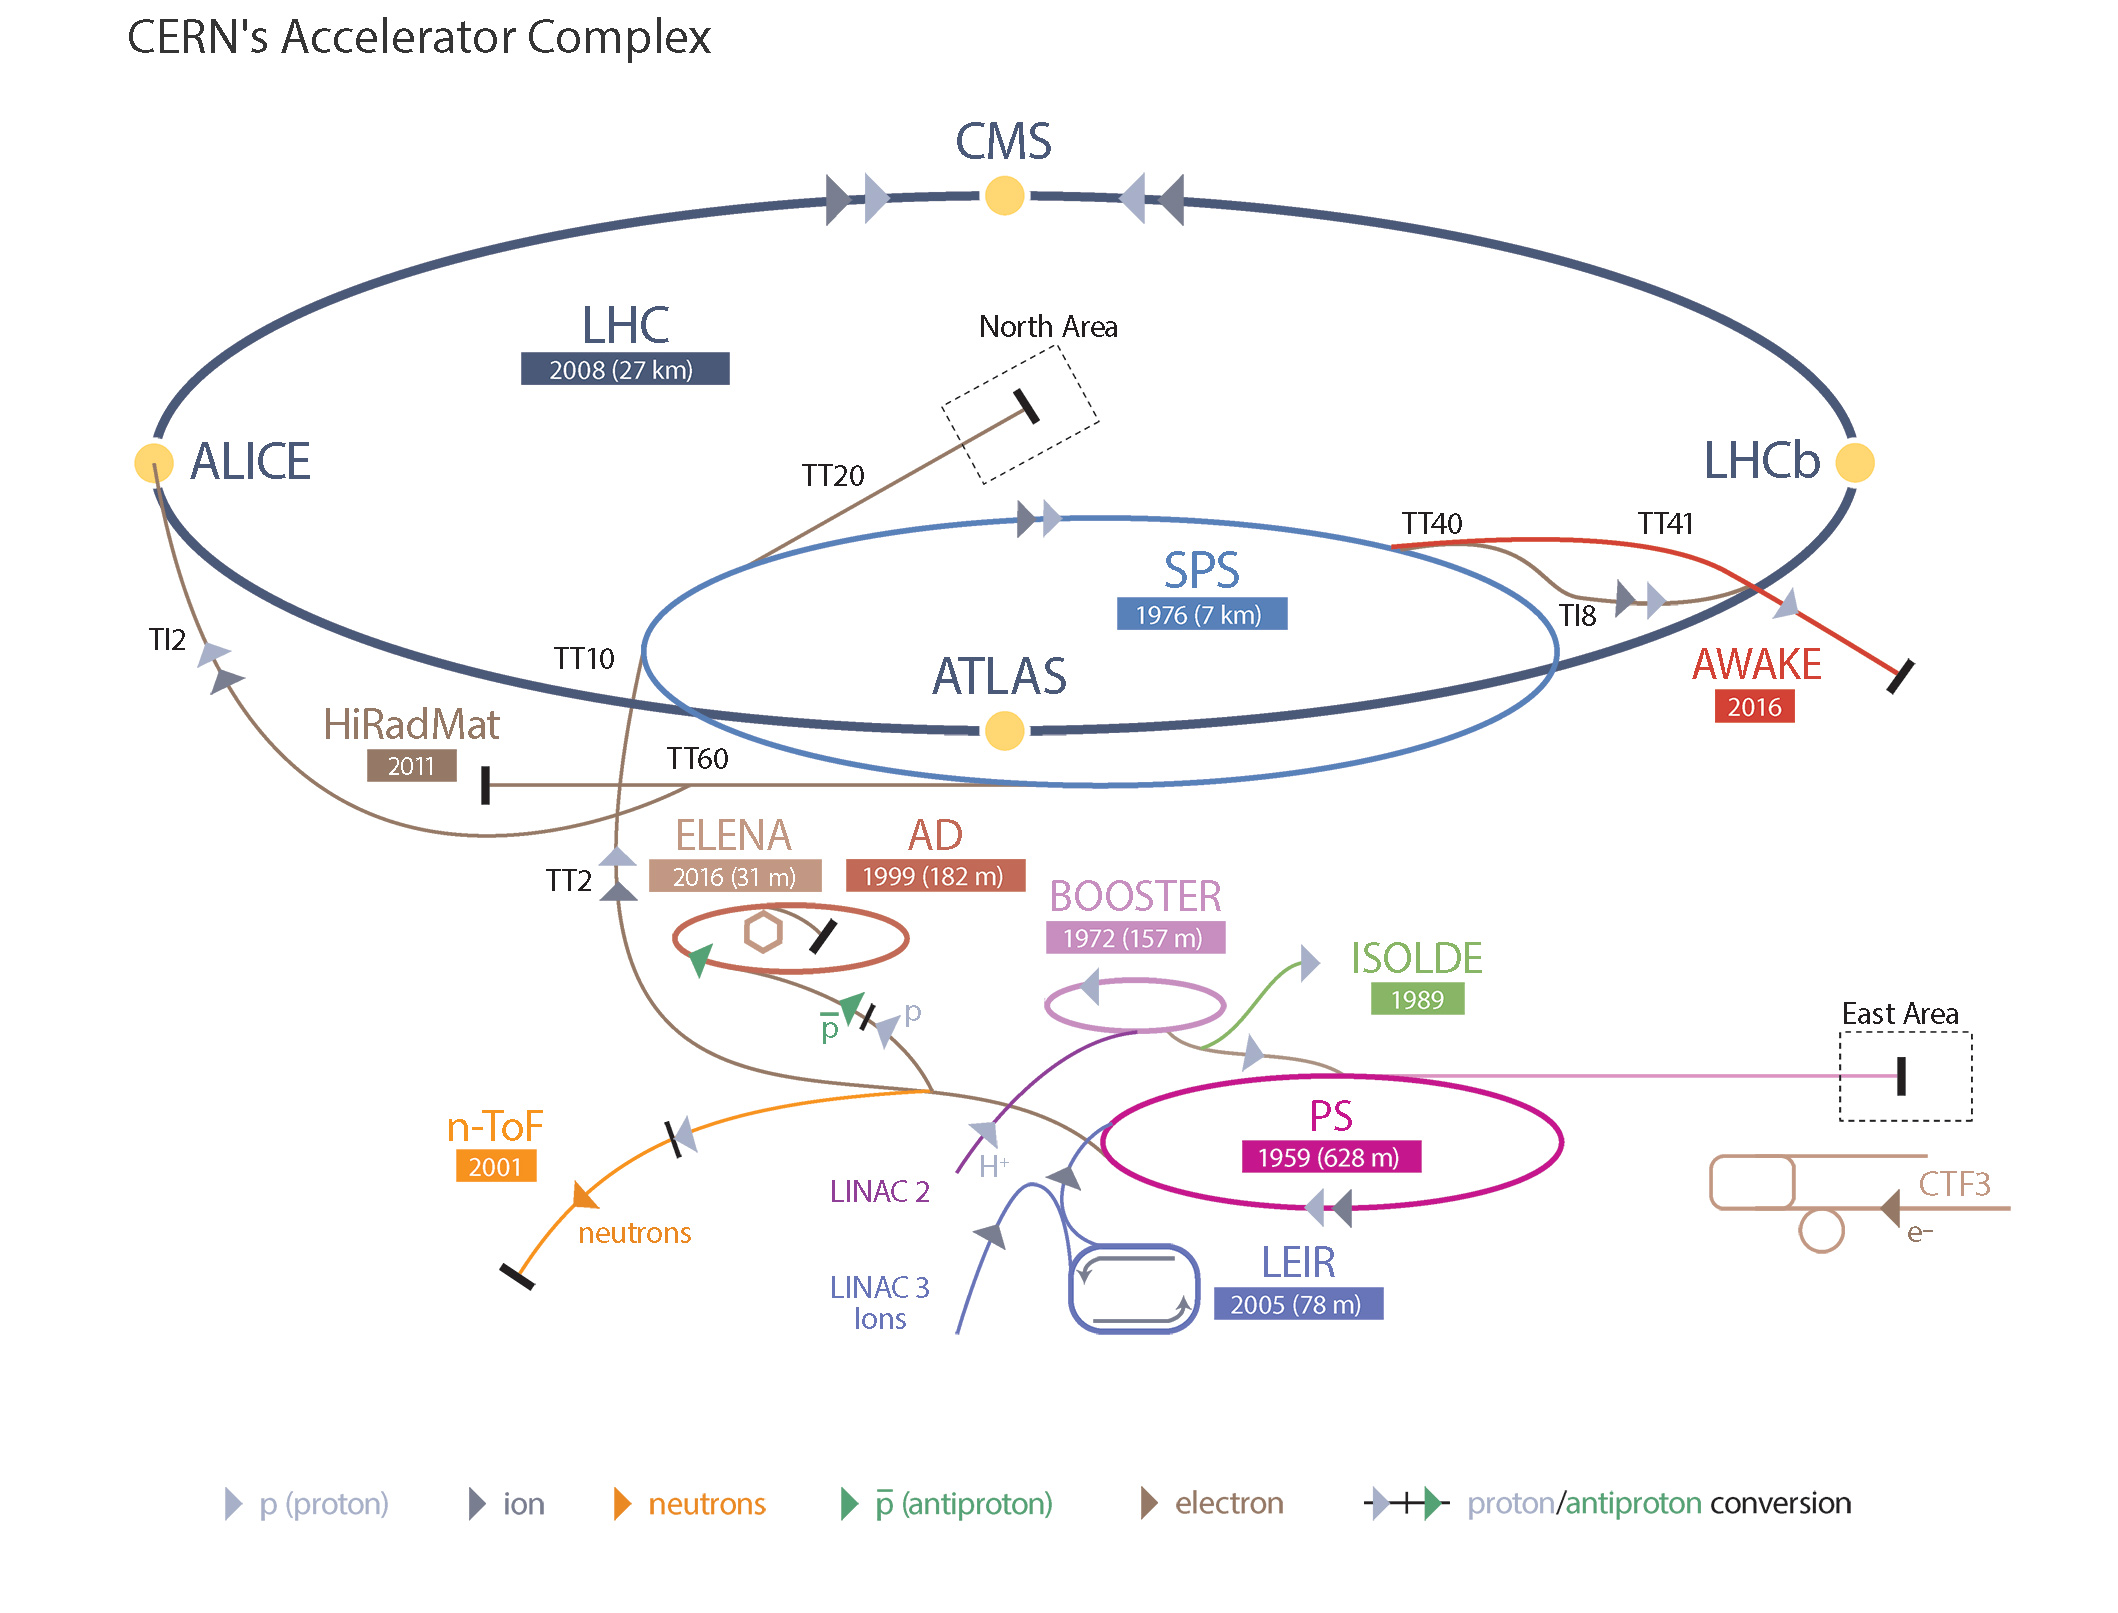
\includegraphics[width=0.75\textwidth]{LHC_default.jpg}
  \caption {Schematic layout of the LHC.}
  \label{lhcmap}
\end{figure}


\section{The LHC}\label{sec:lhc}
The first LHC budget plan was finalised in 1996 and the final cost was completed few years later. 


Now we will talk about the most important parts of the LHC complex.


 
\subsection{The Magnets}\label{sec:magnets}
To keep the beam of protons on a circular orbit LHC needs strong magnets. The proven technology existed since Tevatron and relied on $NbTi$ superconductors. It was decided to use the same alloy for the LHC dipoles that bend the beam and keep the beam on a circular orbit. 

Explain dipole


With ... 1232 dipoles at 8 $T$, which are cooled to below 2 $K$ temperature using liquid Helium, bend the beam, see Fig. \ref{lhcDipole}. The dipole mass is in the so-called Helium bath and is cooled down to 1.9 $K$. Each dipole is 16.5 $m$ (with ancillaries) long and 570 $mm$ in diameter. The dipoles are slightly curved by 5.1 $mrad$ to help a chain of dipoles approximate 360 degrees. A dipole is placed inside of the dipole cryostat

, which is a long cylindrical tube 914 $mm$ in diameter made of low-carbon steel. During the standard data run the vessel operations under vacuum. 


%
%\begin{figure}[H]
%  \centering
%  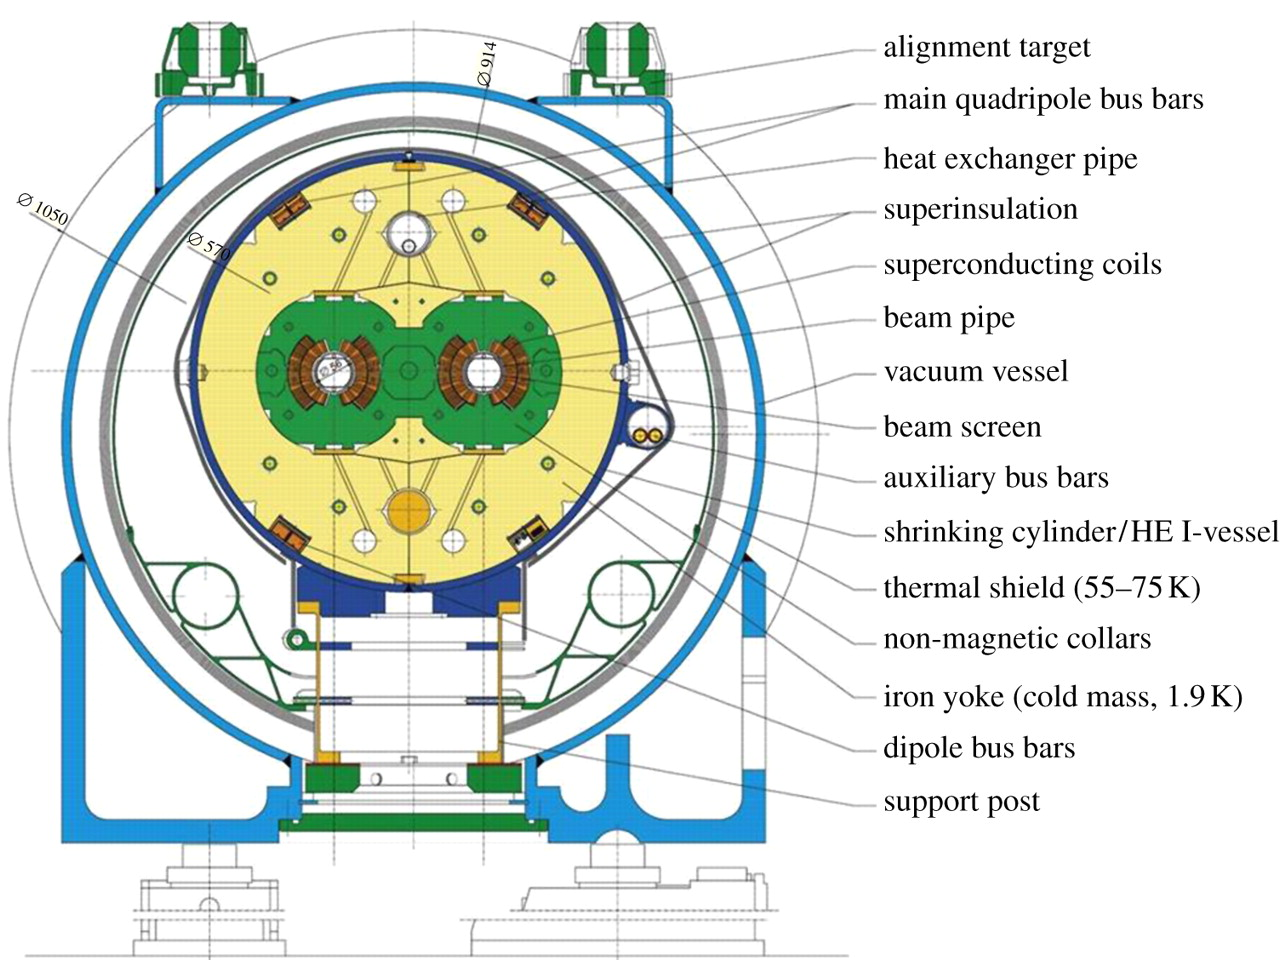
\includegraphics[width=0.9\textwidth]{lhcDipole}
%  \caption[The cross section of an LHC dipole]{The cross section of an LHC dipole.}\label{lhcDipole}
%\end{figure}

To have the right sequence of ideas, it seems to me that the logic should be reversed, and go as (schematically): each dipole has a coil made of cables? the material of cables is carefully chosen [to satisfy these requirements? etc].
    Note that qualitative adjectives like ?carefully? are usually not used in academic writing, because they do not carry information (and here they supposedly did everything carefully).



Each dipole coil is 56 $mm$ in diameter and is made of cables of two types. The cable in the inner layer contains 28 strands 1.065 $mm$ each. The outer layer contains 36 strands 0.825 $mm$ each. 

To correct the beam orbit, about 5000 higher order correcting magnets are used, which are evenly spaced around the circular trajectory of the LHC. 



Also .... magnets...performed with the use of magnets is the beam insertion, which is done at eight insertion locations of the LHC ring. LHC also uses $NbTi$ magnets to accomplish this work. 


\begin{figure}[H]
  \centering
  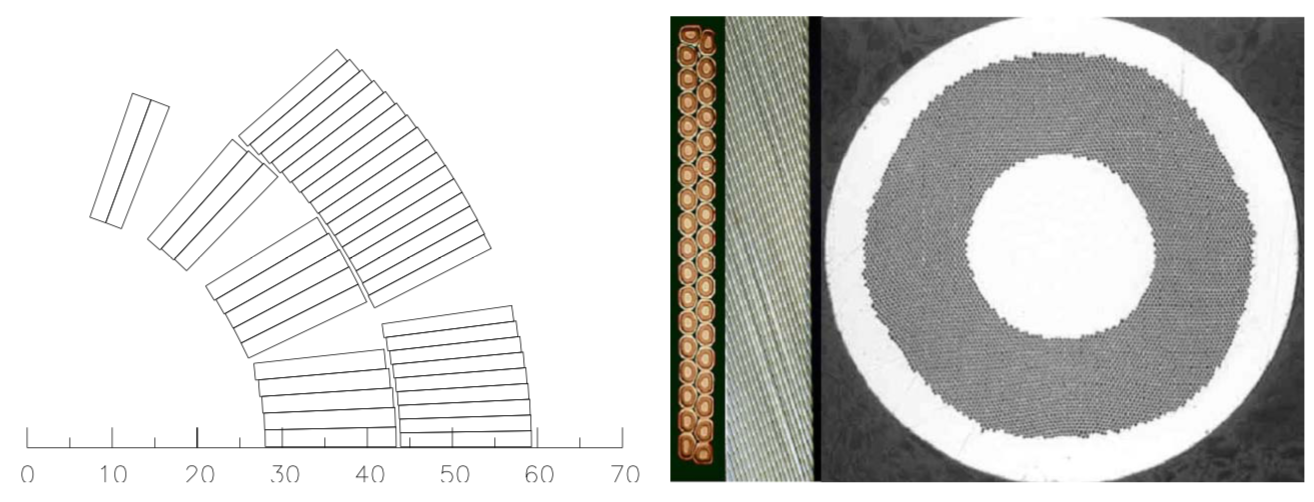
\includegraphics[width=0.9\textwidth]{cables}
  \caption[Cables of the dipole magnet]{Cables of the dipole magnet. Left: cross section view. Right: Strand and cables}\label{cables}
\end{figure}



\subsection{Radio Frequency System}\label{sec:rf}

The beam that comes from injectors are placed???, accelerated and kept on the orbit changing the speed to 

the optimal one with the help of Radio Frequency (RF) cavities (see Fig. \ref{lhc_rfc}). 

The same system is used to correct for injection errors (lower or higher than the optimal speed.....) in the beam direction. 

RF cavities are operating at the 400 $MHz$, which is 10 times more than the revolution frequency of 40 $MHz$ of the circulating beams. 

Four RF cavities grouped together into one cryomodule constitute an accelerating module. If something happens to this module, it can be easily replaced in a short period of time. 


\begin{figure}[H]
\centering
%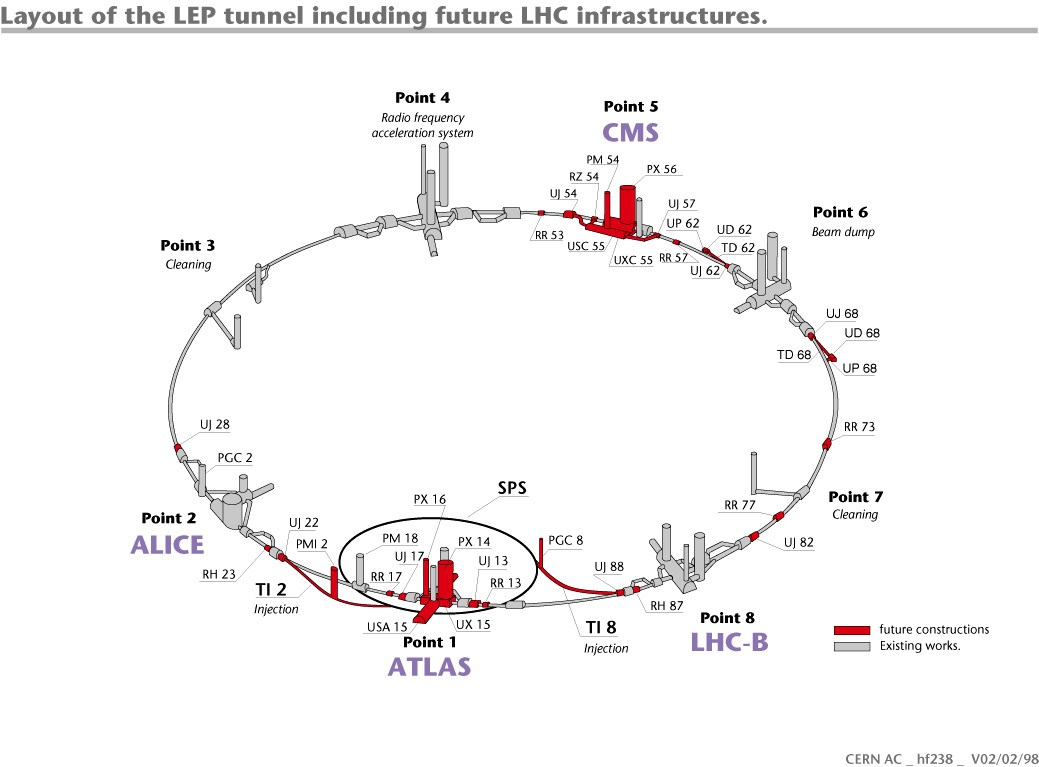
\includegraphics[scale=0.6]{lep}
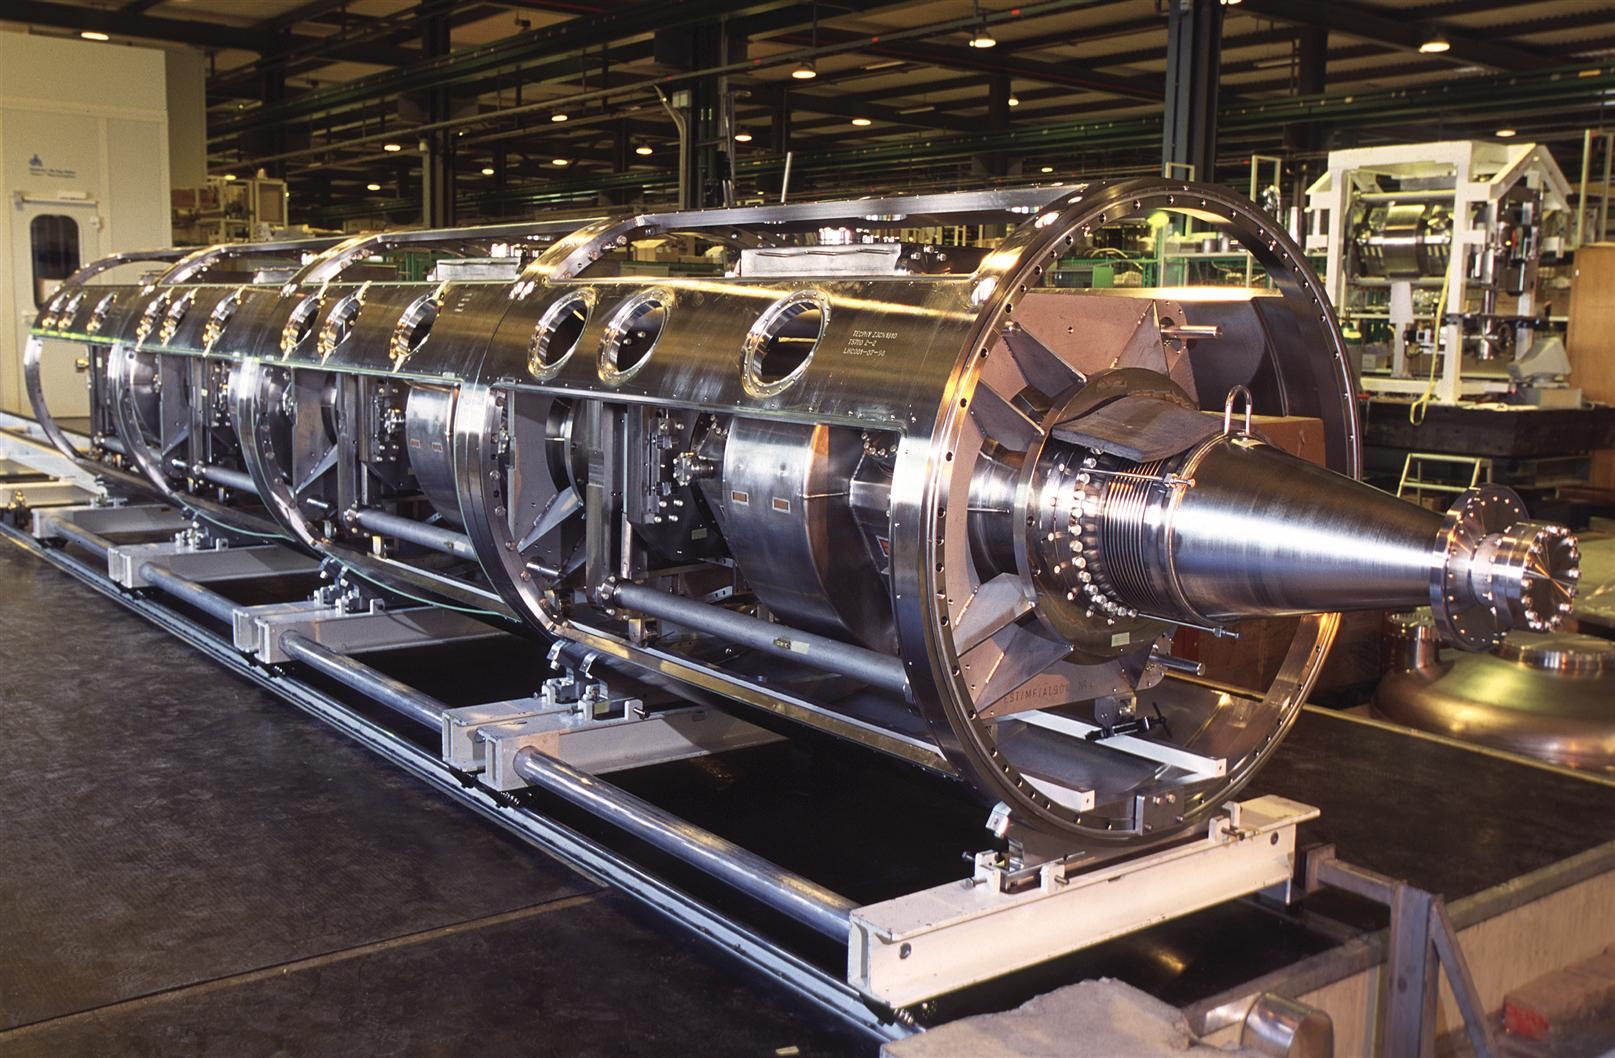
\includegraphics[width=7cm,height=4.2cm]{lhc_rfc}
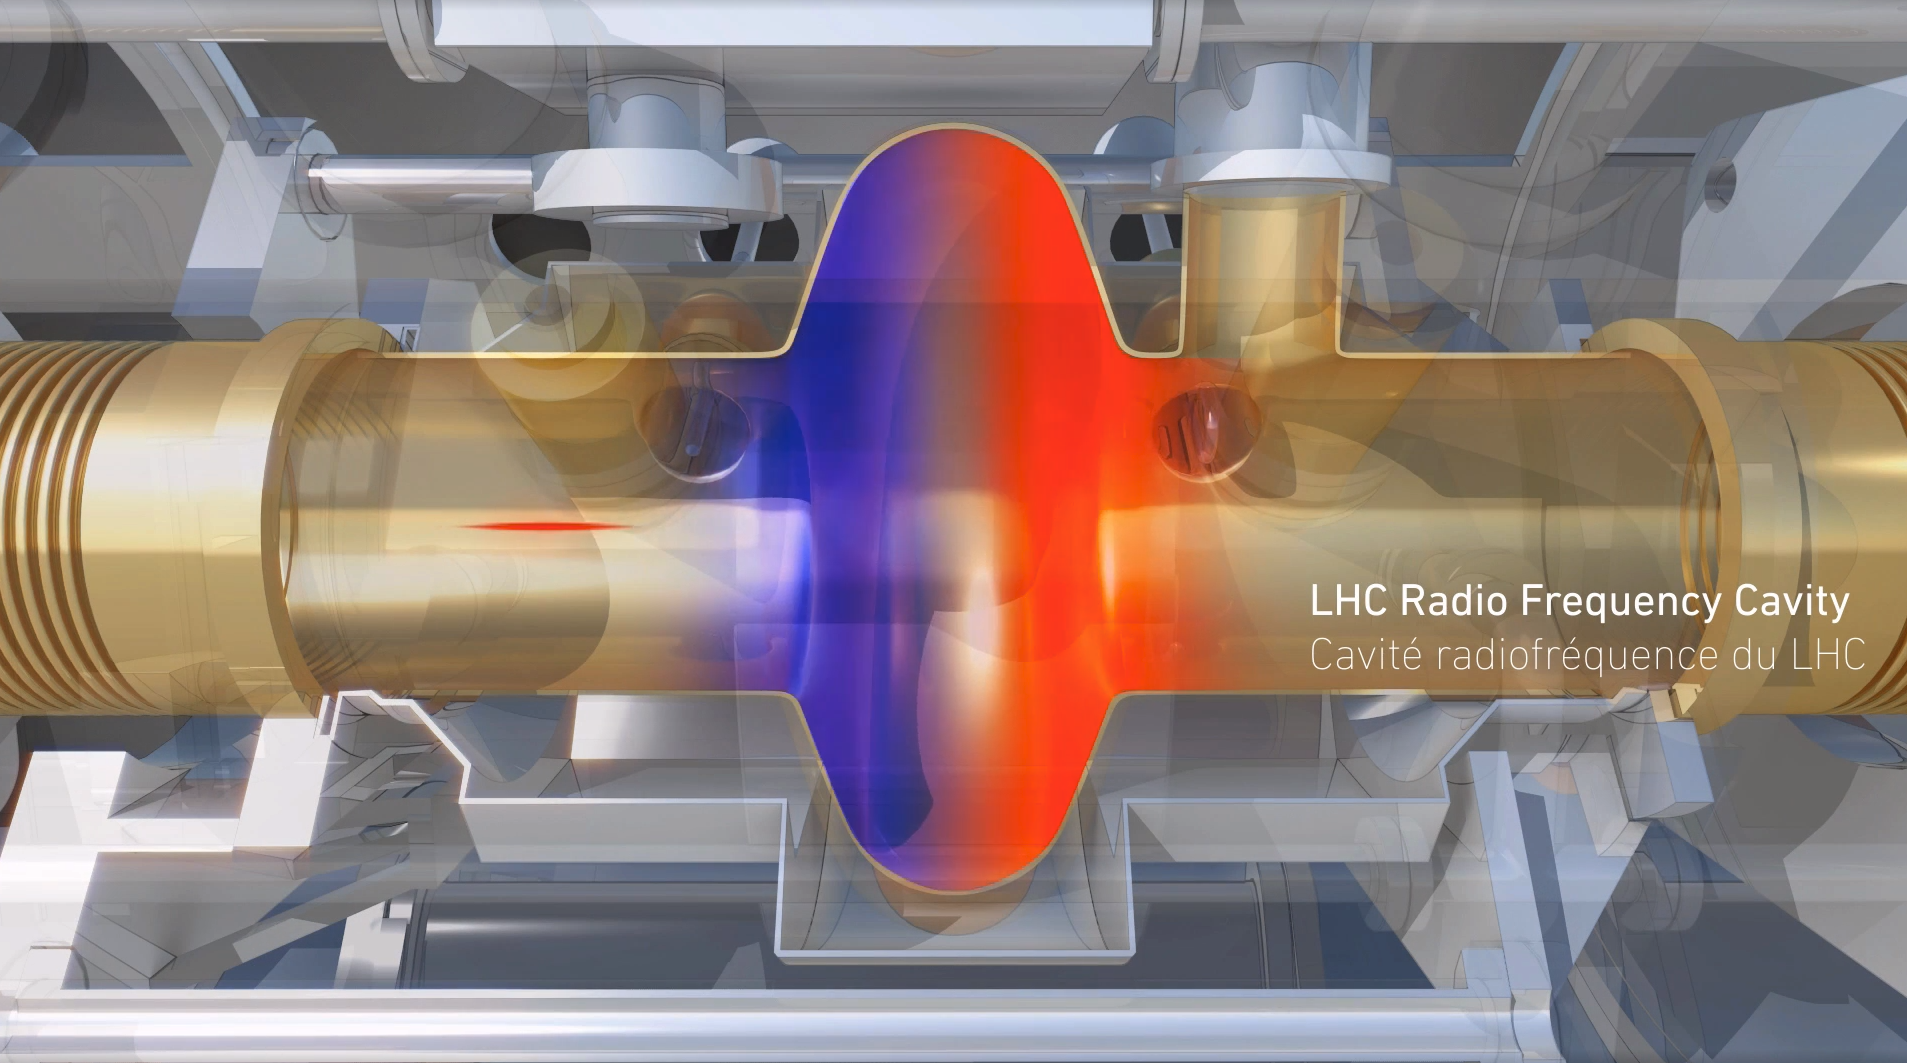
\includegraphics[scale=0.15]{rfc_lhc}
\caption[RF cavities module.]{LHC RF cavities. Left: a cryomodule with four RF cavities. Right: a schematic drawing of a single RF cavity. The colour field is used to highlight the fact of two field of the different polarity. }
\label{lhc_rfc}
\end{figure}


\subsection{Vacuum System}\label{sec:vacuum}


 2. I feel there is a confusion between ?types of systems? and ?systems?. Is there just one system of one type? Is there only one VBS? Or are there many VBSes?
 
 
the vacuum for the beams (VBS). 

%As a convention, taking into account ionisation cross sections for gasses of the interests, cryogenic temperatures are expressed as corresponding gas densities normalised to the hydrogen. 
%VBS, to ensure the 100 hours long run time, requires the equivalent hydrogen densities (EHD) to be below $10^{15} H_2 \frac{1}{m^3}$. To minimise the backgrounds from the experiments, the EHD at the interaction points should be $10^{13} H_2 \frac{1}{m^3}$. Those parts of the beam system, which operate under room temperatures, are under the pressure of $10^{-10}$ to $ 10^{-11}$ $ m$bar. 
%

All the vacuum sections ???which?? are subdivided into smaller modules to allow easy repair and fine tuning. 
VBS, as the most dema???nding in terms of the vacuum quality, the design of the VBS must address a number of challenges, such as synchrotron radiation that may interact with the vacuum chambers of the tunnel, as well as an electron cloud 


 which exists along the circumference of the whole circle of the LHC. After the beam is inserted and is stabilised?????????, the final adjustment of the VBS is needed to guarantee the perfect performance.

Below are the heat sources that degrade the vacuum quality in the beam pipe. The vacuum must exist at 1.9 K:

\begin{itemize}
\item synchrotron radiation (0.2 $W/m$ per beam),
\item energy loss by nuclear scattering (30 $mW/m$ per beam),
\item image currents (0.2 $W/m$ per beam),
\item electron cloud related effects (vary).
\end{itemize}

To reduce effects of the heat sources mentioned above, beam screens are developed (see Fig. \ref{beam_screen}). Screens have elliptical shape, so-called racetrack shape, instead of the circular shape, which provides with the extra space for cooling with the flow of the cold gas.

Finally, since a perfect vacuum does not exist and there is always a small presence of gasses and atoms, the lifetime of the vacuum is mostly determined by the interactions of the vacuum gas nuclei with the protons of the beams. 


\begin{figure}[H]
  \centering
  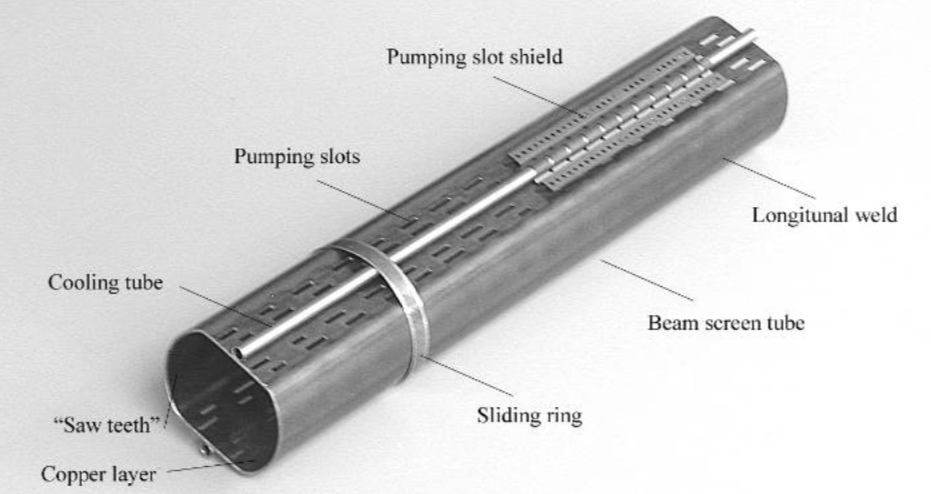
\includegraphics[width=0.7\textwidth]{beam_screen}
  \caption{Beam screen.}\label{beam_screen}
\end{figure}

\subsection{Power??ing}\label{sec:power}
To power the LHC, 1612 electrical circuits are used. The magnets are powered in eight location of the LHC. 
A total of 3286 current leads are needed to connect all the circuits and power cables. More than a thousand of the leads operate between 600 A and 13 kA (see Fig. \ref{13kA_lead}). The other leads work in the range 60 to 120 A. 

\begin{figure}[H]
  \centering
  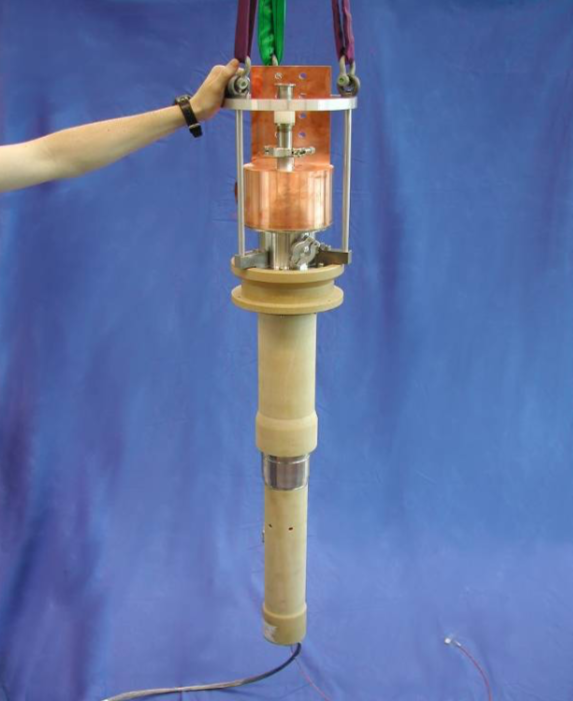
\includegraphics[width=0.5\textwidth]{13kA_lead}
  \caption{13 kA high-temperature superconducting current lead.}\label{13kA_lead}
\end{figure}












\subsection{Cryogenic system}\label{sec:cryogenic}


I think you need to change this subsection to use human-readable, yet precise language. Give basics first. The cryo system is needed to keep superconducting LHC magnets at the appropriate temperature (anything else?) It runs on liquid helium (although it may not be liquid everywhere?). It uses layered design with the temperature becoming progressively colder as you go from outside in for a chilled component such as the magnets. Once you give the basics, you can then give details like surges or perturbations or vertical depth difference.


The cryogenic system (see Fig. \ref{cryo}) must supply 37 Mkg of the LHC magnets within 15 days with the necessary temperatures corresponding to ????? The temperatures vary based on the system by 75 K. 

Since I, as a reader, do not know what this cryo system does exactly from the above, I do not know what pressure
raises and flow surgers you are talking about (pressure of what? flow of what? Why surges and changes?)
  Also I am not sure if ?raises? is appropriate word here. I feel slightly uneasy about it, but maybe I am wrong.
  It is bot clear what is meant by ?the run of the whole LHC?.
  
  
The system must also be able to deal with the fast pressure raises and flow surges, and should be able to recover in a short period of time from such perturbations not to affect the run of the whole LHC. 

? point that had to be addrssed in the cryogenic system design is ?

 important point during the cryogenic design that had to be addressed is the fact that the LHC tunnel is inclined in the horizontal plane by 1.41$^\circ$. This translates to 120 m difference in the vertical location of two diametrically opposite points of the tunnel with respect to the surface level and results in the additional hydrostatic pressure that can affect the flow of the cryogen. ???mention cryogen before
 
 
 To avoid any instability of the LHC work, the gas is transported in the super-heated-vapour state. 

\begin{figure}[H]
  \centering
  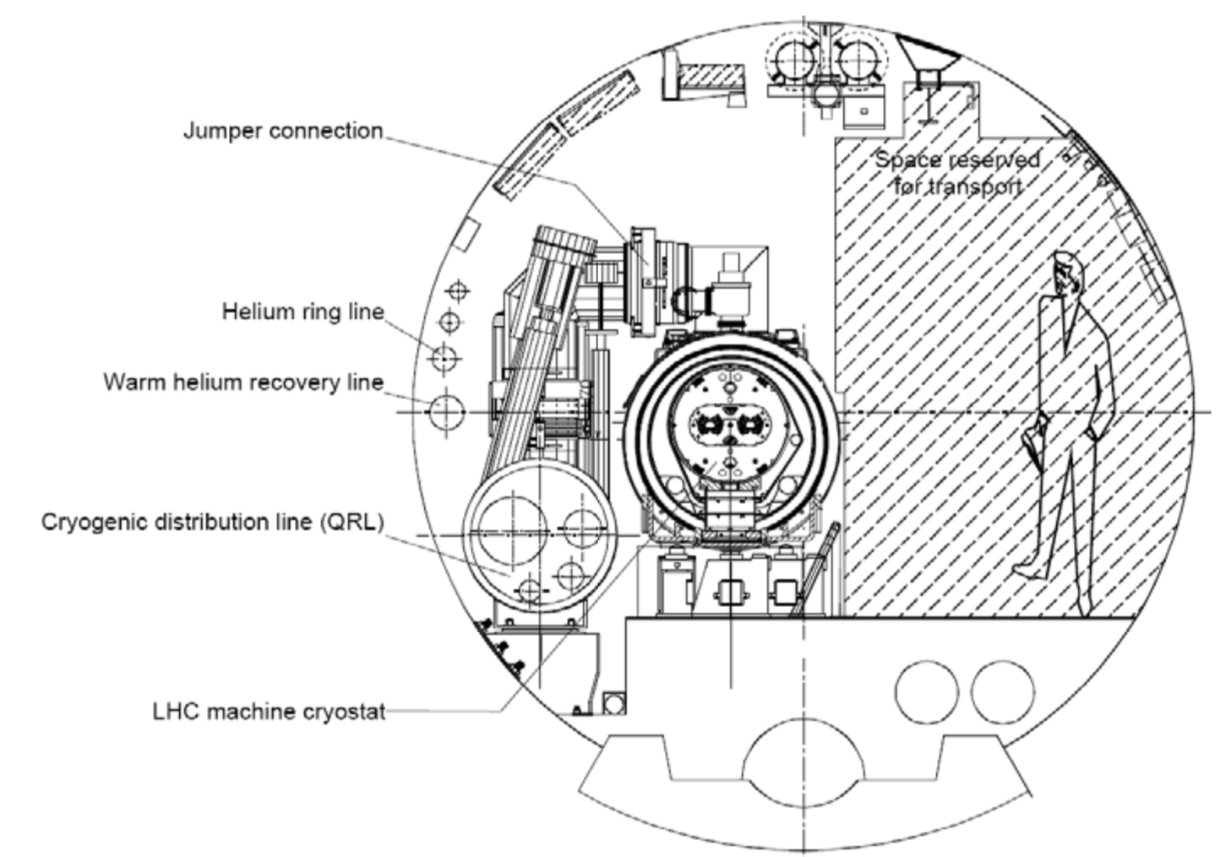
\includegraphics[width=0.7\textwidth]{cryo}
  \caption{Cross section of the LHC tunnel with the cryostat shown at the centre}\label{cryo}
\end{figure}


Since the cost to cool the LHC parts to 1.8 K temperatures is high, several temperature levels are employed (see Fig. \ref{cryo_T_scale}):
 
\begin{itemize}
\item 50 to 75 K for the thermal shielding that protects the dipoles??
\item 4.6 to 20 K for lower temperature interception and to cool the beam screens ??explain THEM
\item 1.9 K for quasi-isotermal helium in the superfluid state to cool magnet masses
\item 4 K for the transportation system that directs the 1.8 K helium from the exchanger to the 1.8 K refrigerator EXPLAIN THEM
\item 4.5 K for RF cavities and lower sections of the high-temperature superconducting current leads
\item 20 to 300 K for upper sections of the high-temperature superconducting current leads
\end{itemize}

\begin{figure}[H]
  \centering
  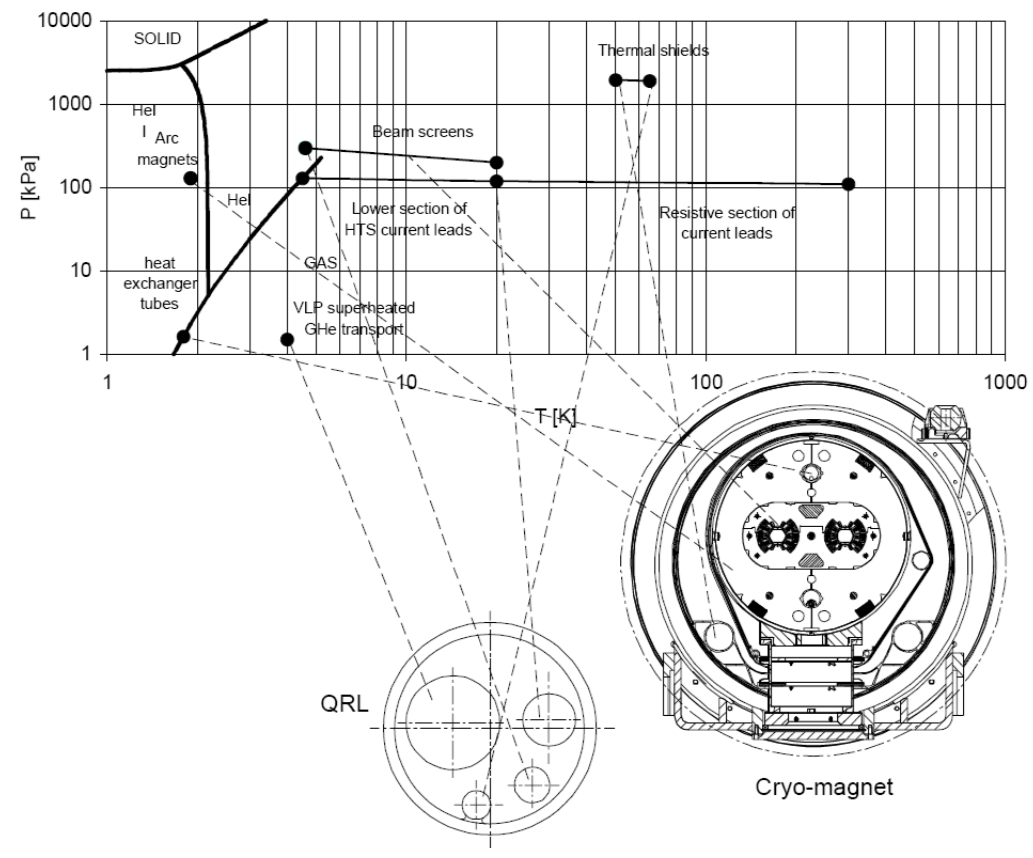
\includegraphics[width=0.7\textwidth]{cryo_T_scale}
  \caption{LHC cryogenic states and the temperature scale.}\label{cryo_T_scale}
\end{figure}


\subsection{Beam dumping system}\label{sec:dumping}

The LHC beam carries a lot of power and a well-designed and reliable beam extraction and dumping system is needed. EXPLAIN

Point 6  INTRODUCE at LHC contains such system, which is able to fast-extract??? the beam in a loss-free way EXPLAIN. The system for each ring comprises:


all of these sound cryptic, I have no idea what are ?dolution kicker magnets? and how they are different from ?kicker magnets? and from ?dilution devices?. I do not know what is a ?septum magnet?. I do not know what is the ?beam dump proper?. All in all I do not understand how it works. You could have simply explained that the beam dump system has a set of magnets dedicated to steer the beam/bunches out of their circular path in the LHC beampipe and direct them into a massive tatget of steel and concrete where the beam energy/particles is absorbed and dissipates. You can also mention that the beam 


%\begin{itemize}
%\item 15 kicker magnets for extraction 
%\item 15 steel septum magnets around the Point 6 interaction point
%\item 10 modules of the dilution kicker magnets
%\item the beam dump proper with the associated steel and concrete for shielding
%\item dedicated dilution devices 
%\end{itemize}

\subsection{Beam injection system}\label{sec:injection}

This logic structure looks reverse to me. Consider first discusssing the acceleration chain, that culminates with injection into the LHC beam pipe. Then one would discuss what systems are needed (cryo, voltage, dump, etc). 


What is ?injection?? Even a small change to ?The proton beams are injected into the LHC at two points?? would dmake it more clear.

 is done at two points of the LHC and for both circulating beams separately: at Point 2 and Point 8. EXPLAIN
 
 The beam comes to the insertion point from outside and below the machine level EXPLAIN. 
 
 A series of magnets and a kicker then deflects the beam horizontally and vertically to place the beam on the LHC orbit. To protect against the problematic??? injections and malfunctioning of the kickers EXPLAIN BEFORE, a series of the collimators correct the incoming beam. 

\subsection{LHC injection chain}\label{sec:injection_chain}

Many problems here.
1. ?To place the beam, the protons have to travel?.  How do protons place the beam? This does not make literal sense.
2. What is hydrogen bottle?
3. ?protons from the hydrogen bottle extracted from the hydrogen gas? sounds confusing. Are they from the hydrogen bottle or from the hydrogen gas?
4. ?have to travel a long pass?, how do you travel a long pass?
5. ?put into bunches? -> ?arranged into bunches?


To place the beam at the final LHC orbit, the protons from the hydrogen bottle extracted from the hydrogen gas have to travel a long pass during which they are put into bunches and accelerated to the nominal collision speed. 

\begin{figure}[H]
  \centering
  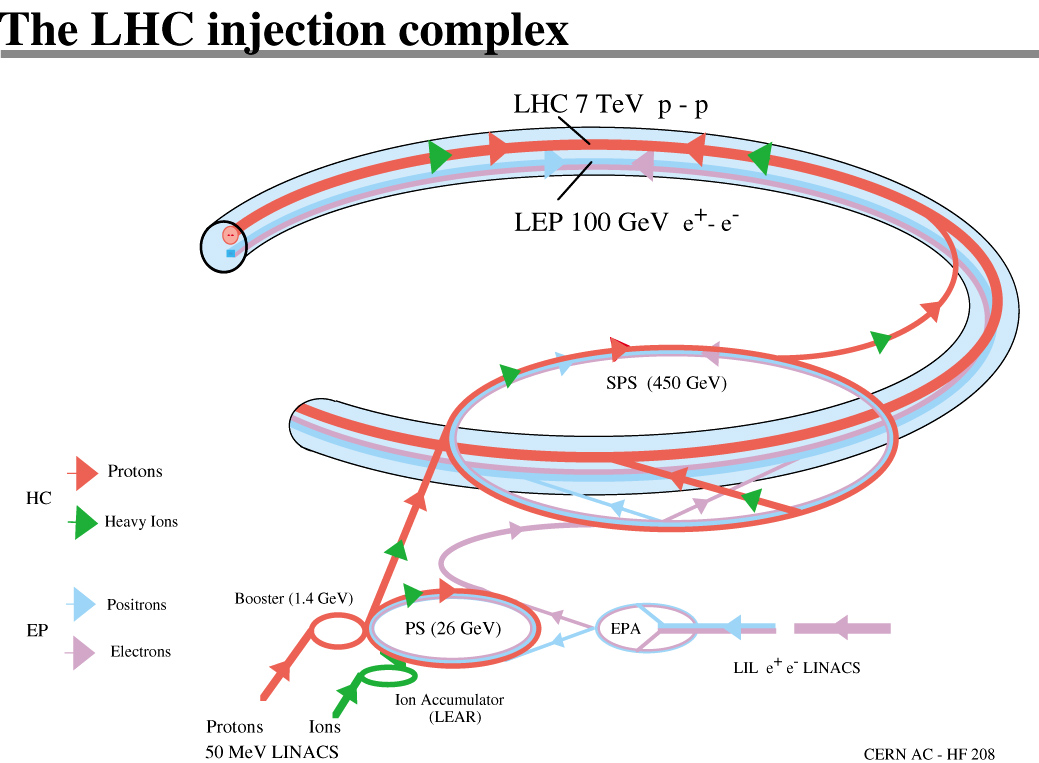
\includegraphics[width=0.7\textwidth]{lhc_complex}
  \caption{LHC injection complex.}\label{lhc_complex}
\end{figure}


The accelerator complex consists of: LINAC, Booster, Proton Synchrotron, Super Proton Synchrotron, and finally, the LHC main ring (see Fig. \ref{lhc_complex}). 

The whole LHC complex has to satisfy requirements of the final ring, such as:
\begin{itemize}
\item the beam emittance EXPLAIN has to be compatible with the small aperture of the LHC superconducting magnets
\item the effect of the synchrotron radiation EXPLAIN has to be taken into account when calculating the required cryogen needs for the intensity of the incoming beam
\item the beam-beam interactions that enhance the betatron oscillations should be limited EXPLAIN
\item in the injector the space-charge WTF?? limits have to be taken into account
\end{itemize}

\section{The CMS experiment}

Overall, this section has to be required significantly. 
   Even if you look at the subsections, you have just two (as opposed to the LHC  description that has many subsections), and nowhere there is a section that indicates that this is about the CMS detector.
   But more than that, you need to figure out a logical way to present informtion about the CMS experiment in the right order. The logical blocks might include:
  - general comments that the CMS experiment revolves around the CMS deteector which is a general purpose particle deteector placed in a cavern around one of the interaction points at the LHC, and is capable of detecting and measuring properties of particles of all sorts with the exception of neutrinos, etc.
  - requirements that drove design choices for the CMS deteector can be discussed
  - somewhere a section on physics objects where you discuss that there are tracks, there are jets, there are b-jets, what it means an isolated lepton, what it means missing momentum, and so forth. For example, Ekaterina has a section on particle flow, if I remember right, where she discusses that. Or you can have a section that just discuses the proton-proton collisions environment and explains that many particles created in collisions are unstable and decay right away. What is observable in an experiment such as CMS is longer-lived or stable particles. These include electrons, muons, photons, and some ground state hadrons. At the same time, energetic quarks or gluons hadronize and can be seen in a particle detectors as jets of hadrons (so define jets here). Same for tau leptons, we detect them either as electrons/muons, or hadronic jets. Etc. If you have such a conceptual paragraph here, some time later you can have a particle flow discussion when it is time to be more specific. But discussion at this level above would allow you to then discuss the requirements on CMS design using terms like b-jets or isolated leptons.
  - the coordinate system section is good to have.
  - the CMS detector section
  - consider also discussing the trigger system after discussing all subdetectors, this could be part of the CMS detector section.
  
  
The total inelastic cross section of the proton-proton interaction at $\sqrt{s}=13$ is about 70 $m$b. The detectors observe the event rate of nearly $10^{9}$ inelastic events per second.

This flow of data is too large to be stored, and also, does not contain that many event of interest.
 
 
 Hold on, I am suddenly disoriented. You have not even introduced CMS, but you are already talking about the trigger system, pileup, etc.

 
 
  Therefore, the trigger system must reduce the event rate to manageable 100 events per second. 
  
  In addition, a pile up DEFINE (PU) of 20-200 events overlaid with the event of interest will be expected, 
  
  which results in about 1000 particles produced every 25 ns. 
  
  INTRO ALL SUBDETECTORS
  
  
  
  
  All sub-detectors of CMS (see Fig. \ref{cms_cross_section}), thus, have to be able to work fast and in a good synchronisation with each other. 


\begin{figure}[H]
  \centering
  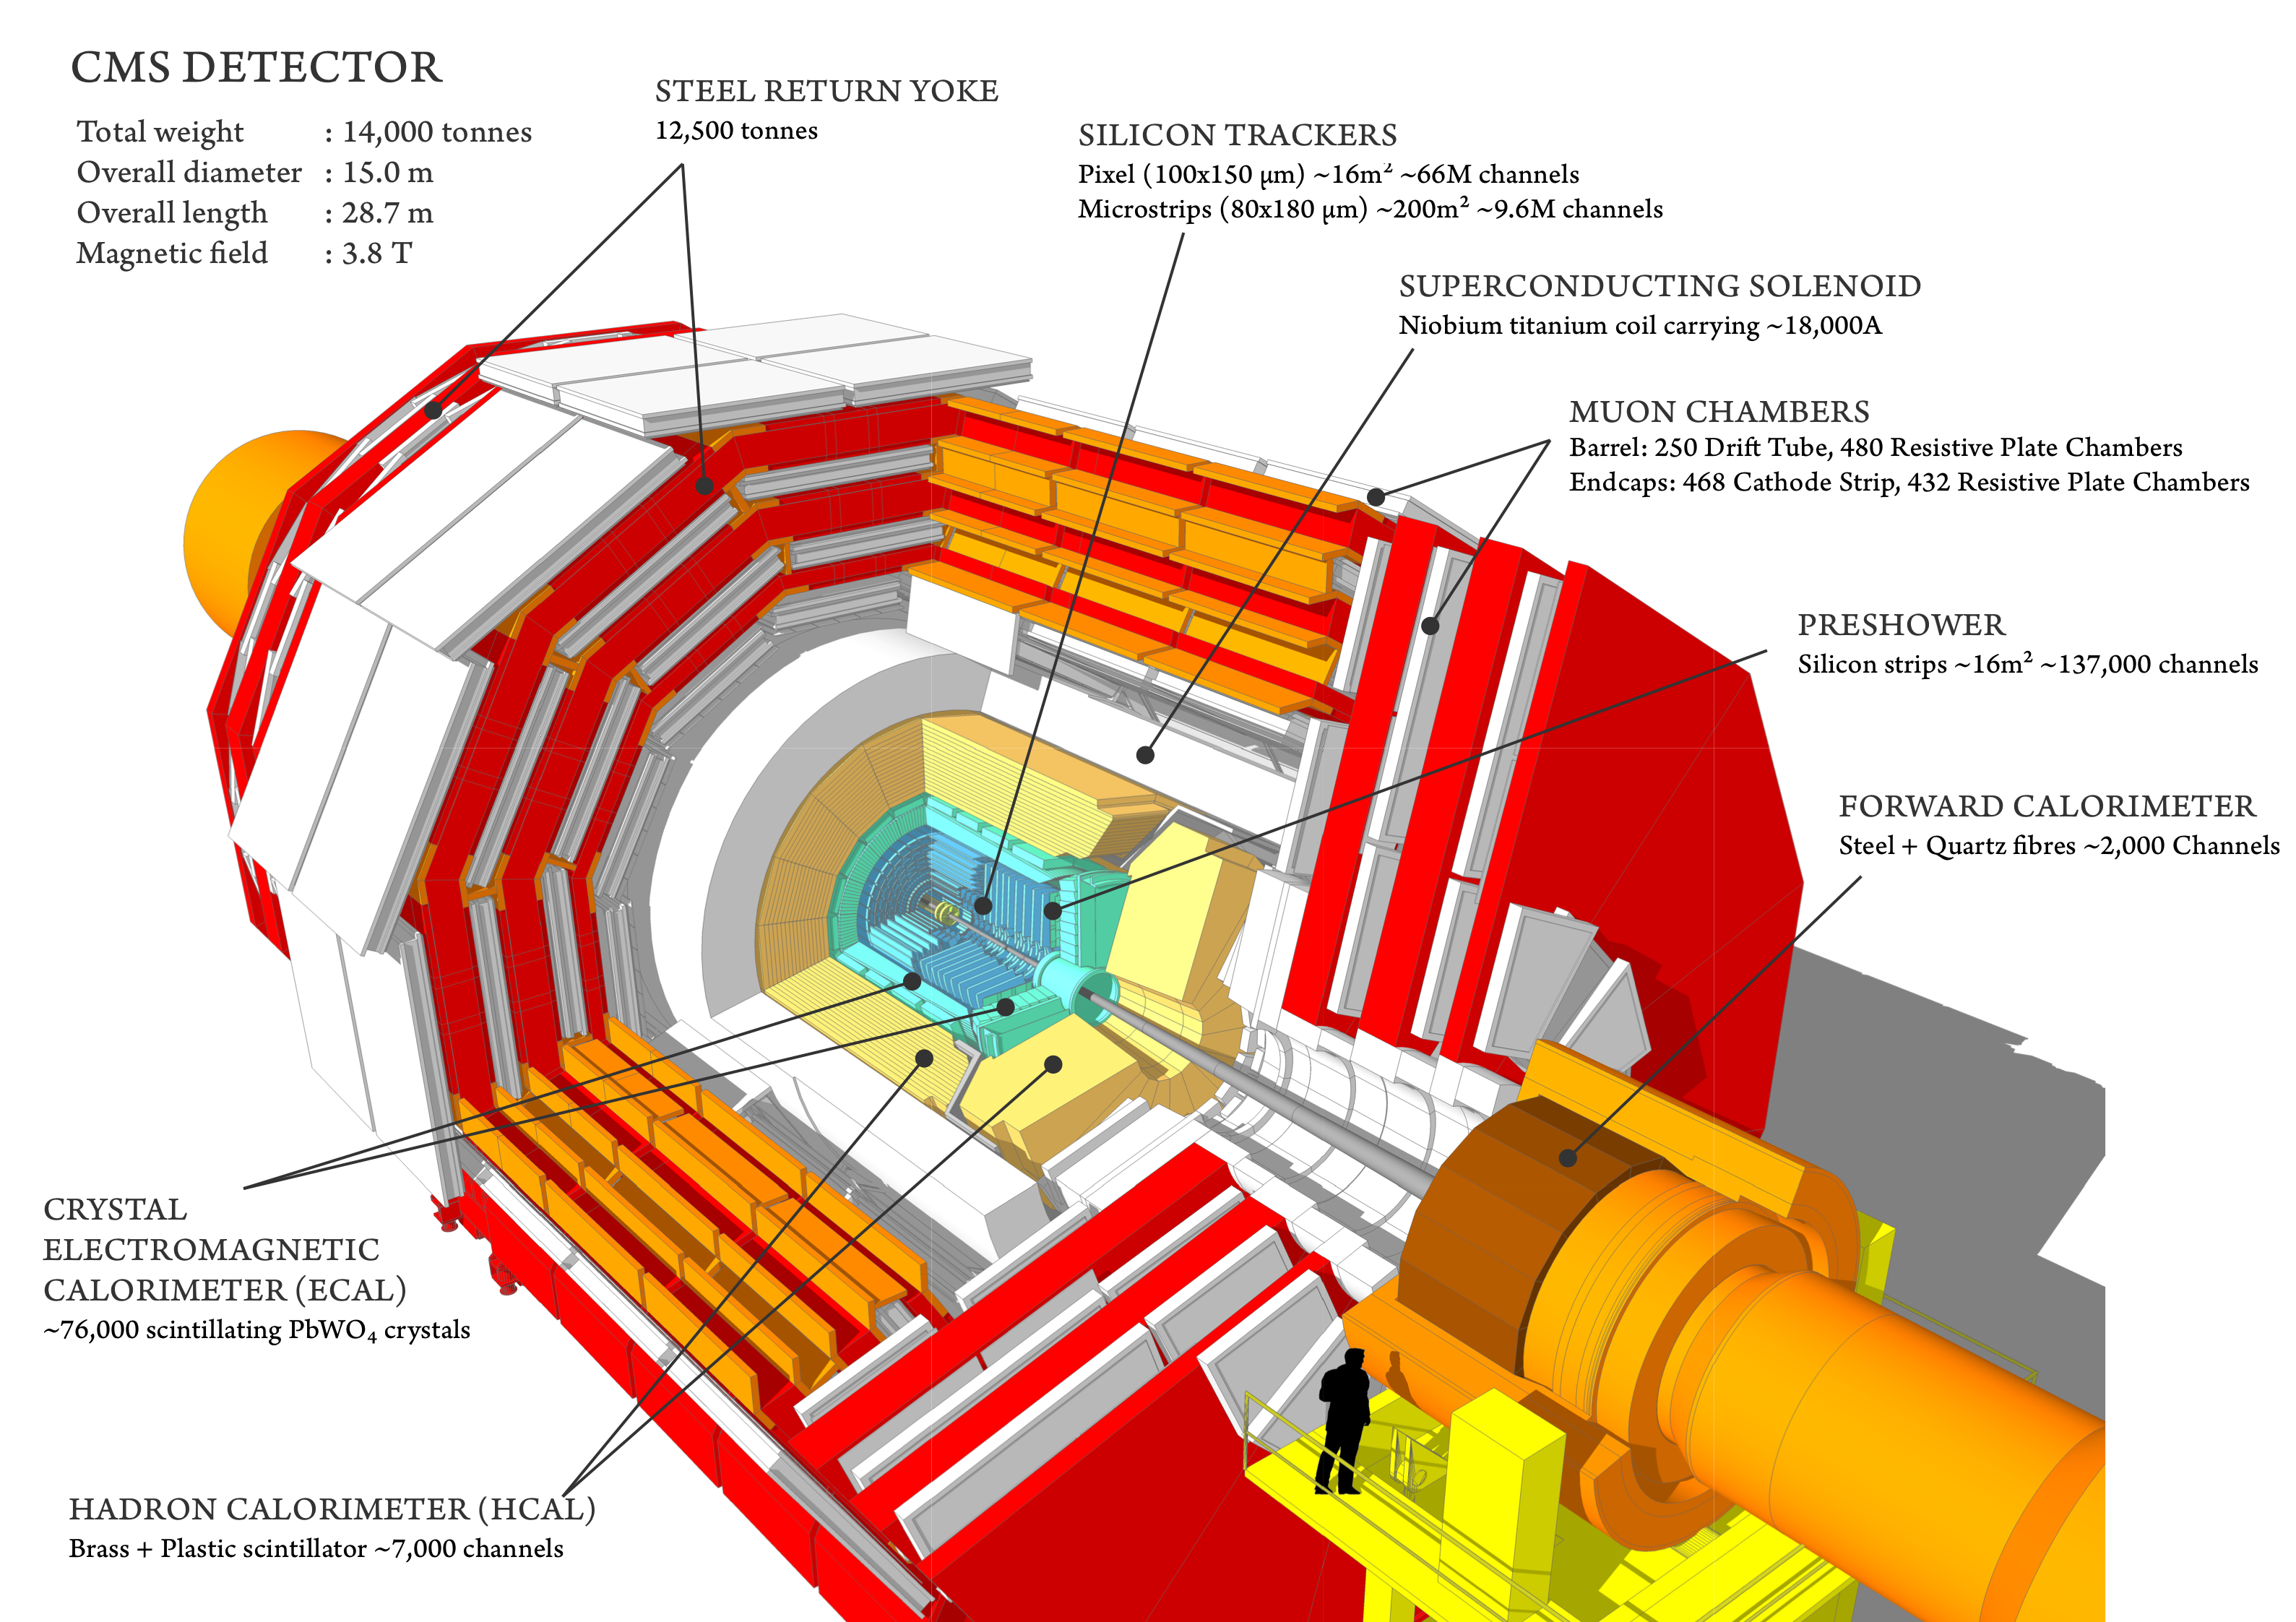
\includegraphics[width=0.9\textwidth]{cms_cross_section}
  \caption{CMS experiment with all sub-detectors shown.}\label{cms_cross_section}
\end{figure}

\subsection{The CMS detector specifics}

1. ?One can? appears unnecessary. You just summarized. So just say: The following list summarizes the main challenges and requirements that the LHC has faced.
2. But the above still won?t be good. Listing challenges and requirements in one list is odd (apples and oranges). Also, ?requirements that the CMS has faced? does not sound right.
3. What you want to convey, perhaps, is that to achieve its physics goals, or successfully complete its physics program, or such, the CMS detector is designed to have: good momentum resolution, etc etc, or the design goals for the CMS detector required for success of the CMS phusics program were?


One can summarise all challenges and requirements that the CMS has faced in the following list:

You mention throughout this bullet list CMS systems: tracker, ECAL, HCAL, and what requirements are imposed on their design. But the reader at this point has no idea what these systems are.

Generally, a lot of stuff is undefined here and in the above bullets. Maybe every single thing would be painful to  define, but a non-collider physicist will be lost quicjly here. 
  What is diphoton, dijet mass? 
  What is ?missing transverse mass??
  What is a jet? What is a b-jet?
   What are isolated leptons and photons?
  You are thrusting a reader into a jargon-rich environment without preparation.


\begin{itemize}
\item good muon momentum resolution over the momentum scale covering almost a TeV range, good dimuon ??????resolution at the 100?????/ GeV, and a capability to determine correctly the charge of the highly energetic muon all the way up to 1 TeV
\item good momentum resolution of the charged particles in the inner tracker. CONNECTION Emphasis on the efficient $\tau$ lepton and b-jets reconstruction
\item good performance of the electromagnetic calorimeter (ECAL), with the particular attention to the diphoton mass resolution, ability to reject efficiently $\pi^0$ EXPLAIN, ability to identify isolated photons and leptons
\item good missing transverse mass and dijet-mass resolution, which depends heavily on the performance of the hadronic calorimeter (HCAL)
\end{itemize}

The first part, the bullet list of the design goals, seems not connected in any way to the detector description that follows. Not even clear to me why these two are in the same section.


The CMS design has been driven by the needs to have a large bending power, which is to be provided by the superconducting magnet, to be able to disentangle ............??????/various charged particles. 

The paragragh structure is odd: you have one paragraph discussing the magnet + strip tracker, and a separate paragraph is fully devoted to pixels. Odd grouping.






The size of the magnet is 13 m in length and 6 m in inner diameter. 4 T solenoid provides 12 Tm bending power. The inner  DEFINE diameter is large enough to host the inner tracker and the ECAL. To address the high multiplicity problem???, the CMS inner tracker uses 10 layers of the silicon microstrip detectors. The inner barrel contains four layers of strips and the outer barrel has six layers. Each silicon sensor is 320 $\mu m$ in height and a specifically designed overlay of strips provides a spatial resolution of 13-38 $\mu m$. About the same resolution is achieved by the other tracker. The whole tracker contains 15148 silicon modules with the 9.3 million strips. Tracker provides the experiments with the tracks information left by the charged particles traversing its material. 

To further improve the impact parameter determination and secondary vertex reconstruction, three layers of the silicon pixel detector are inserted near the interaction region. Pixel detector ADD DETAILS OR REMOVE SOME FROM THE INNTER TRACKER is composed of 1440 silicon pixel detector modules organised in three concentric cylindrical layers, and also two disks in the forward regions. 


PURPOSE OF ECAL The ECAL technology is based on the on the lead tungstate crystals ($PbWO_4$). The ECAL measures the energy deposited by photons and electrons. ECAL contains 75848 crystals where the energy showers???? will be produced by the particles releasing their energy when interacting with the material of the crystals. Before the ECAL, a preshower system is placed to reject $\pi^0$. 

1. How does the preshower system ?reject? pi0?  Actually, data from the preshower subdetector allow us to identify pi0 (and thus reject pi0 candidates in the measurements where they are a background).
2. The preshower subdetector is there only in the endcap, by the way.


It contains layers of lead radiators followed by layers of the silicon strips to initiate???? and subsequently to measure the energy of the particle. The ECAL measured energy of the particles is a function of the stochastic term (S), noise (N), and a constant term (C). 

It is not a function of the stochastic term, etc. It is a function of energy, and the expression contains the stochastic term, the noise term, etc.
  Also, have the ?:? at the end, and ?.? at the end of the equation.
  
  
\begin{equation}
  \left(\frac{\sigma}{E}\right)^2 = \left(\frac{S}{\sqrt{E}}\right)^2 +
  \left(\frac{N}{E}\right)^2 + C^2
  \label{eq:ecal}
\end{equation}

The ECAL 
magnet
then
HCAL system

 which is based on the brass/scintillator sampling hadronic technology. HCAL measures energy of particles made of quarks. 
 
 What does it mean ?later?? Later usually refers to time sequence.

Why is tail-catcher italicized, are you consistently using this method to introduce new terms? But you do not explain this term here. (You had plenty of unknown terms before, like kickers or tracker, and never italicized those).
   Also, in general, I do not understand this sentence, what does it mean ?leaving 11 hadronic interactions?, how ?11? is to be interpreted (a lot? little?), etc.
   
   
   Central part is later covered by the $\textit{tail-catcher}$ leaving 11 hadronic interaction lengths to the particle interactions.  
Further, the forward calorimeter is used to ensure the coverage in $\eta$ up to 5. Note, that the coverage of ECAL and HCAL are about up to $\eta=3$.  

Is this forward calorimeter part of HCAL or not? If it is, then the next sentence seems to contradict this eta=5. If it is a different subdetector, I do not know whether to expect that it uses the same technology, has the same reoslution, uses the same principles, or not.


If you want to list the eta coverage of different subdetectors, then list this in the right place (e.g. HCAL measures energy of hadrons with the eta range ? ? etc.), not tucked in at the end as an afterthought.




Additional dedicated detectors such as  CASTOR, ZDC, etc, ensure that the detector has almost a full $4\pi$ coverage. 

The paragraph content seems unbalaanced. HEre you switch to other detectors, and then you come back to the HCAL.

HCAL does not fully absorb energy of the the particles traversing its medium, except very low energy particles, thus the energy of the particles is sampled to estimate the total amount.  

I am missing something her. The HCAL contains vast majority of showers initiated by hadrons in full. Because it has 11 radiation lengths in depth. Which is because it was designed as a sampling calorimeter, with a lot of absorber. Why do you say that HCAL only fully absorbs energy for vey low energy particles? This doesn?t make sense.
   Also, energy of the particles is sampled is very unclear. In fact, what is sampled is the energy of the shower developing through HCAL that was initiated by the original paricle we wnt to measure. Outer HCAL is located outside of the magnet.

   
   
   
Overall, the CMS detector is 21.6 m in length and 14.6 m in diameter. The weight of the whole construction is near 12 500 tons. ECAL covers more than 25 radiation lengths, HCAL, from 7 to 11, depending on the $\eta$ region. 
It is not clear that that?s the best way to summarize, listing ECAL and HCAL radiation lengths (it is also not trivial presentation, because the reader may not know that ECAL has 25 radiation lengths for photons and electrons, but very little radiation lengths with respect to hadrons).


The superconducting magnet of CMS provides the experiment?????/ make smooth..........??????? is operated at the 4.7 K temperature. 



This discussion of the muon system needs to be improved and made uniform with the discussion of other subdetectors in structure and content. As it is, it reads as an assorted set of sentences, unconnected.
  Also, notice that in some cases you ovewhelm the reader with numbers (like the numbers of crystals or strip sizes,) and in others you hardly mention any numbers of that sort (HCAL, muons).
  
  
  , a magnet yoke is made of five barrel wheels is used for the magnetic flux return and serves as a support for the embedded muon system, which is located outside of the ECAL and HCAL systems. Muons are energetic enough to traverse the ECAL and leave the detector. Tracks in the muon system will be used to reconstruct standalone muons, and in combination with the tracker, to reconstruct the global muons.  


\subsection{CMS coordinate system}


This sounds awkward. Consider instead something like simply ?In this section we introduce the coordinate system used in CMS?. You di not need to say that you will use rapidity and pseudorapidity in te analysis section. But you do need to define the directions of the origin of the coordinate system and the directions of the X, Y, and Z.

We will use rapidity and pseudorapidity many times in the analysis section of the thesis. The coordinate system employed by the CMS uses the rapidity, y, and pseudorapidity, $\eta$. They are derivatives of the log functions of the energy and a projection of the momentum of the beam/?????? on the z axis and the angle $\theta$ with respect to the beam axis (see Fig. \ref{coord} \ref{MonroyMontanez:2639240}):


ON THE PIC explain what are eta1, eta2, phi1 and phi2? or FIND A NEW PIC


\beqn
y=\frac{1}{2}ln\frac{E+p_z}{E-p_z} \qquad \eta=-ln \left(tan\frac{\theta}{2}\right)
\label{eqn:eta}
\eeqn


\begin{figure}[h!]
  \centering
  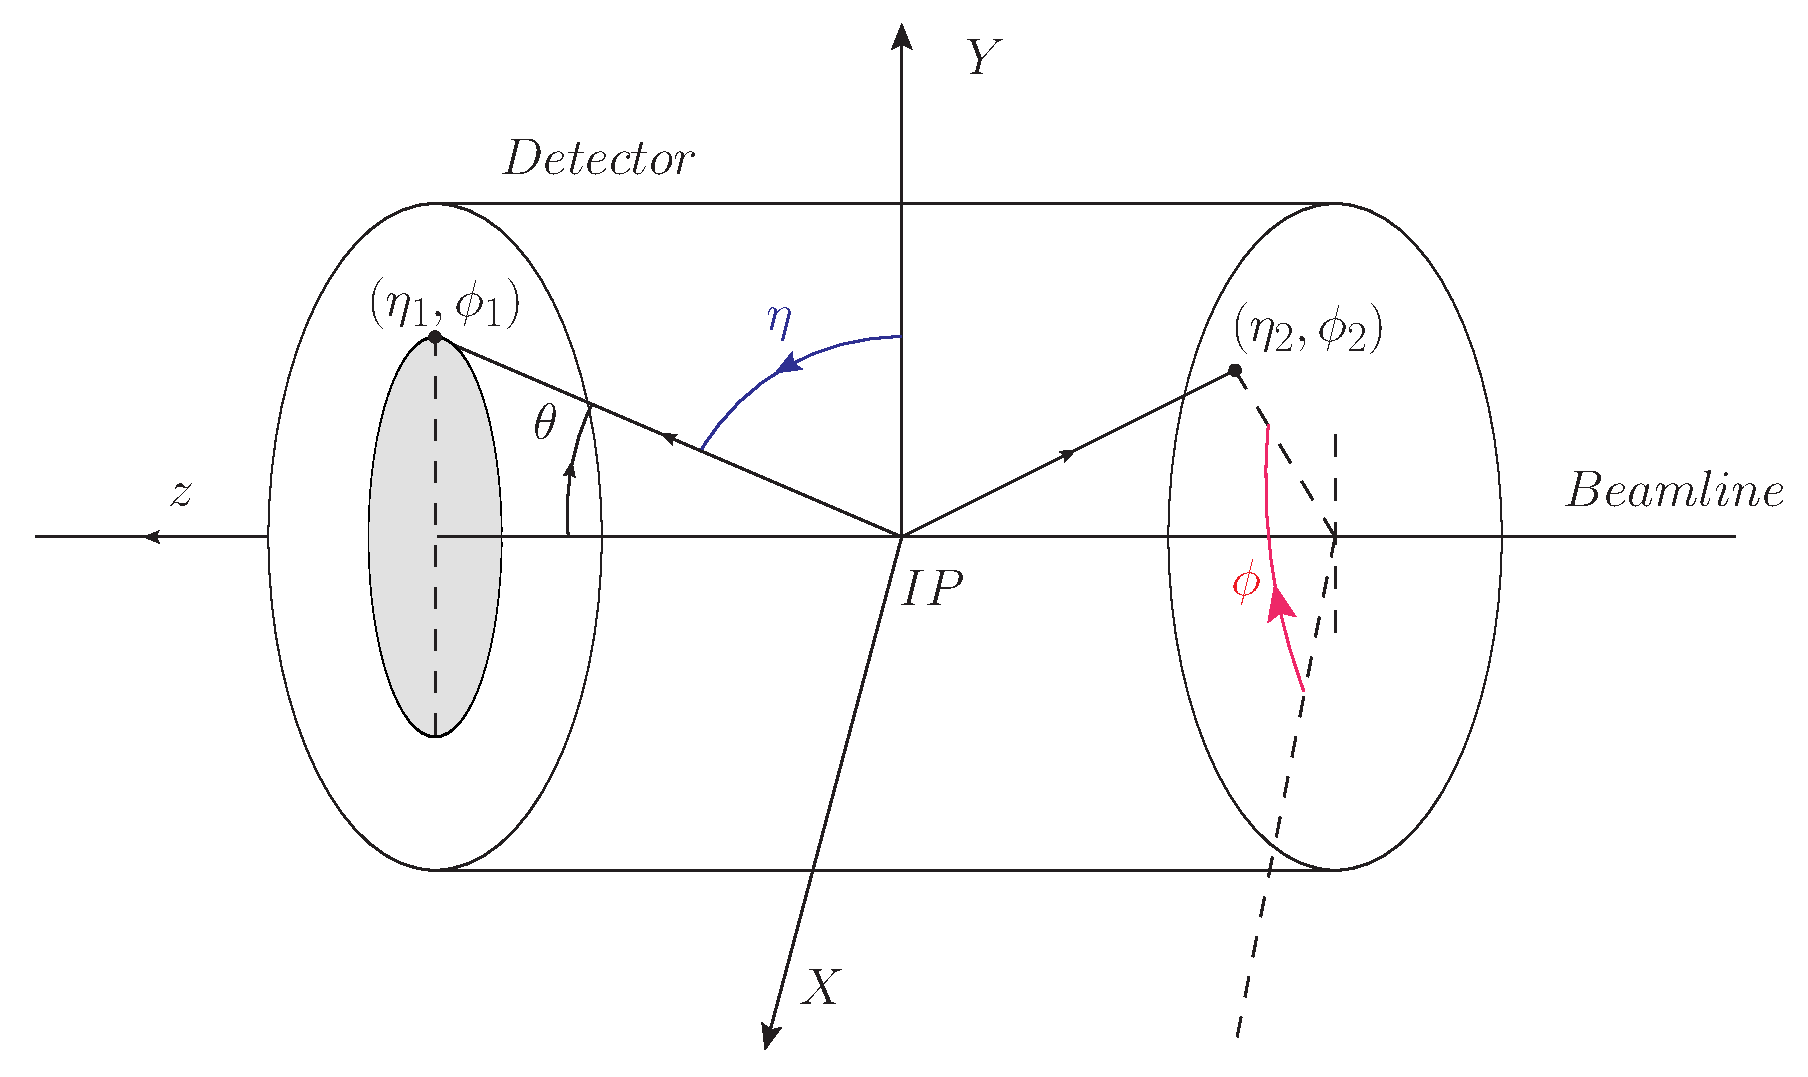
\includegraphics[scale=0.4]{coord}
  \caption[Coordinate system of the CMS detector]{Coordinate system of the CMS detector.}
  \label{coord}
\end{figure}

